\documentclass[journal]{vgtc}                % final (journal style)
%\documentclass[review,journal]{vgtc}         % review (journal style)
%\documentclass[widereview]{vgtc}             % wide-spaced review
%\documentclass[preprint,journal]{vgtc}       % preprint (journal style)
%\documentclass[electronic,journal]{vgtc}     % electronic version, journal

%% Uncomment one of the lines above depending on where your paper is
%% in the conference process. ``review'' and ``widereview'' are for review
%% submission, ``preprint'' is for pre-publication, and the final version
%% doesn't use a specific qualifier. Further, ``electronic'' includes
%% hyperreferences for more convenient online viewing.

%% Please use one of the ``review'' options in combination with the
%% assigned online id (see below) ONLY if your paper uses a double blind
%% review process. Some conferences, like IEEE Vis and InfoVis, have NOT
%% in the past.

%% Please note that the use of figures other than the optional teaser is not permitted on the first page
%% of the journal version.  Figures should begin on the second page and be
%% in CMYK or Grey scale format, otherwise, colour shifting may occur
%% during the printing process.  Papers submitted with figures other than the optional teaser on the
%% first page will be refused.

%% These three lines bring in essential packages: ``mathptmx'' for Type 1
%% typefaces, ``graphicx'' for inclusion of EPS figures. and ``times''
%% for proper handling of the times font family.

\usepackage{mathptmx}
\usepackage{graphicx}
\usepackage{times}
\usepackage{float}



%% We encourage the use of mathptmx for consistent usage of times font
%% throughout the proceedings. However, if you encounter conflicts
%% with other math-related packages, you may want to disable it.

%% This turns references into clickable hyperlinks.
\usepackage[bookmarks,backref=true,linkcolor=black]{hyperref} %,colorlinks
\hypersetup{
  pdfauthor = {},
  pdftitle = {},
  pdfsubject = {},
  pdfkeywords = {},
  colorlinks=true,
  linkcolor= black,
  citecolor= black,
  pageanchor=true,
  urlcolor = black,
  plainpages = false,
  linktocpage
}
\usepackage[hyphenbreaks]{breakurl}

%% If you are submitting a paper to a conference for review with a double
%% blind reviewing process, please replace the value ``0'' below with your
%% OnlineID. Otherwise, you may safely leave it at ``0''.
\onlineid{0}

%% declare the category of your paper, only shown in review mode


%% allow for this line if you want the electronic option to work properly


%% In preprint mode you may define your own headline.
%\preprinttext{To appear in an IEEE VGTC sponsored conference.}

%% Paper title.

\title{World Soccer Analytics}
%\subtitle{Visual Analytics project, A.Y. 2017/2018}

%% This is how authors are specified in the journal style

%% indicate IEEE Member or Student Member in form indicated below
\author{Angelo Catalani, Alessandro Lo Presti}
\abstract{
Soccer is one of the most popular sports in Europe and the Americas whose origin is in China during the 2nd and 3rd centuries BC.\\The history of modern-day soccer was established in 1863 when eleven representatives from London clubs and schools met at the Freemason's Tavern to set up common fundamental rules.\\FIFA was established in the year 1904 and it organized the first world cup in Uruguay in 1930.\\The goal of the project is to combine automated analysis techniques with interactive visualizations to show the diffusion of world soccer across the world and a comparative analysis among the national teams from the 1873 to 2018.
}
%%%%%%%%%%%%%%%%%%%%%%%%%%%%%%%%%%%%%%%%%%%%%%%%%%%%%%%%%%%%%%%%
%%%%%%%%%%%%%%%%%%%%%% START OF THE PAPER %%%%%%%%%%%%%%%%%%%%%%
%%%%%%%%%%%%%%%%%%%%%%%%%%%%%%%%%%%%%%%%%%%%%%%%%%%%%%%%%%%%%%%%%
  \teaser{
 \centering
 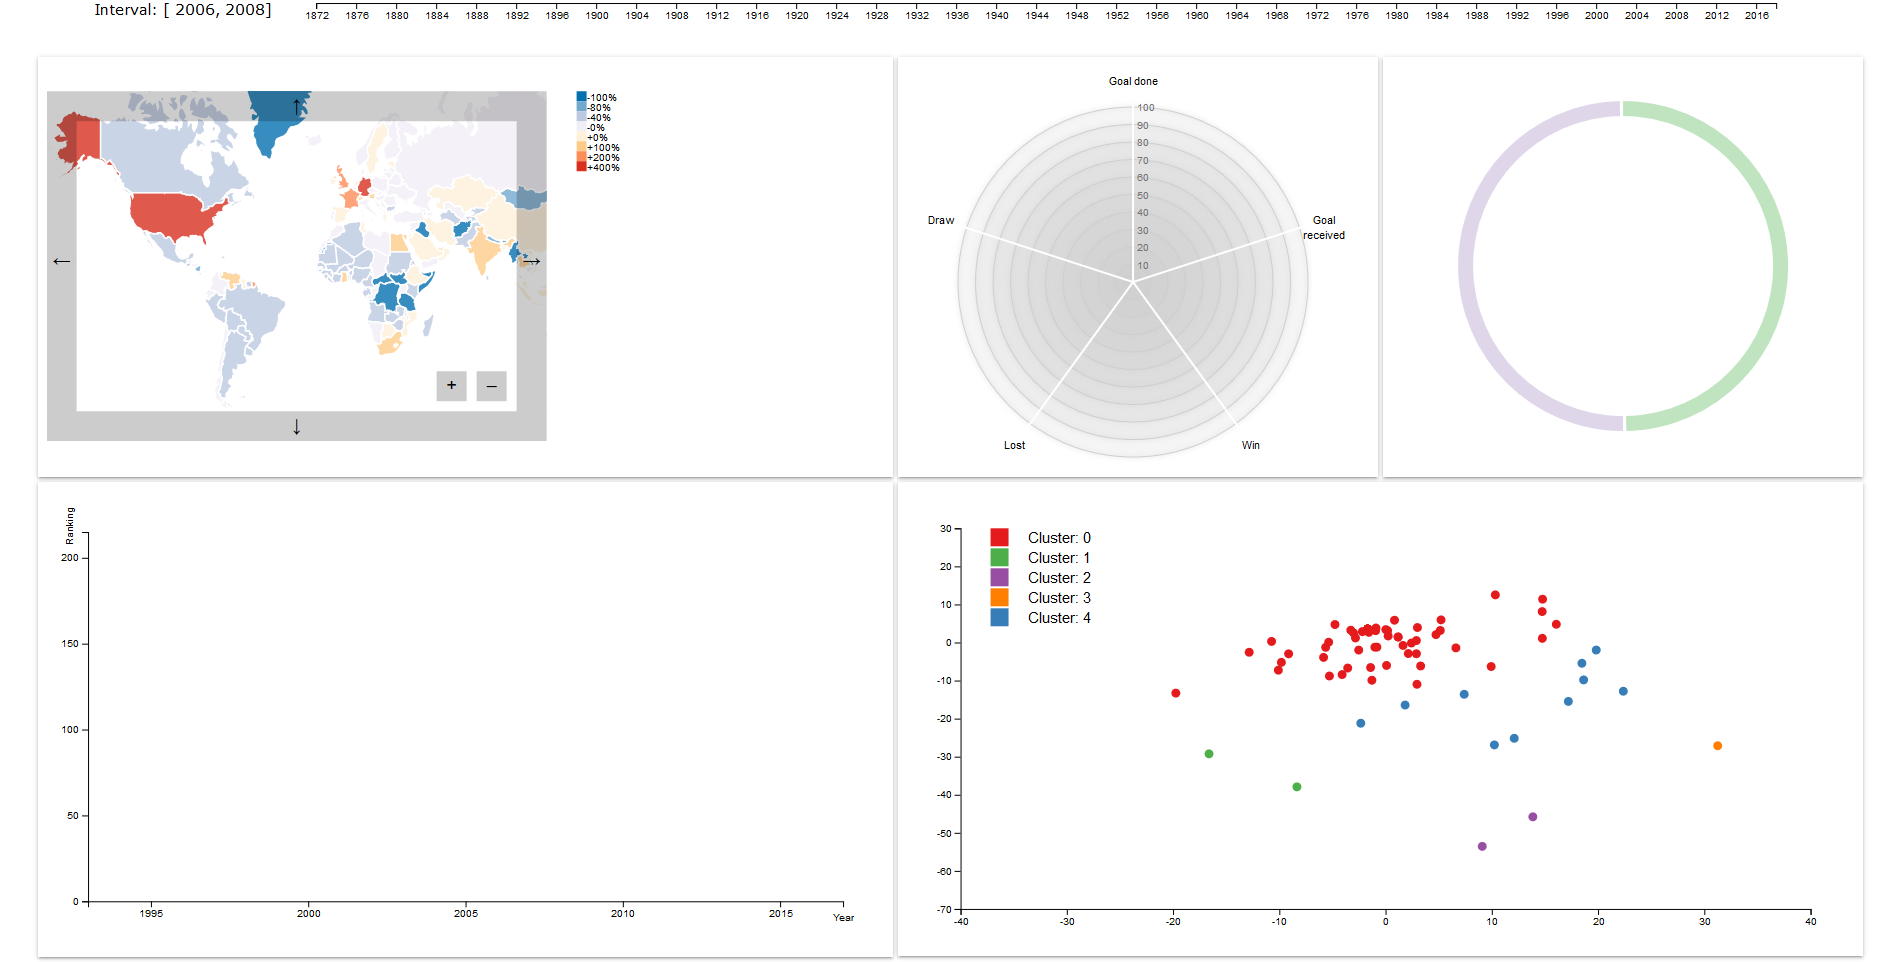
\includegraphics[width=16cm]{view}
  \caption{The whole project in a picture}
  }
\begin{document}

%% The ``\maketitle'' command must be the first command after the
%% ``\begin{document}'' command. It prepares and prints the title block.

%% the only exception to this rule is the \firstsection command
\maketitle
\section{Introduction}
This project contains the following interactive visualizations :
\begin{enumerate}
\item Choropleth Map: the matches played in a given country and to select a team for the other plots
\item Radar Chart: general statistics (win, lost, draw, goal done, goal received) about the selected teams
\item Chord Diagram: the relationships of the selected teams in terms of wins when they played against
\item Line Chart: rank of each team according to the FIFA Ranking
\item Scatter Plot: the results of MDS and K-means
\item Time Bar to specify the time frame of the data displayed by the Choropleth Map, Radar Chart and Chord Diagram.
\end{enumerate}



\section{Data}
We have taken into consideration two datasets: 'International Football Results' and 'FIFA/Coca-Cola World Ranking'.
\subsection{International Football Results}
This dataset was downloaded from Kaggle.\\It includes 39.669 results of international football matches  from 1872 to 2018.\\The features of each result of the dataset taken into consideration are:
\begin{enumerate}
\item \texttt{date}: date of the match
\item \texttt{home\_team}: name of the home team
\item \texttt{away\_team}: name of the away team
\item \texttt{home\_score}: full-time home team score including extra time, not including penalty-shootouts
\item \texttt{away\_score}: full-time away team score including extra time, not including penalty-shootouts
\item \texttt{tournament}: name of the tournament (Friendly,FIFA World Cup,UEFA Euro Qualification,...)
\item \texttt{country}: name of the country where the match was played
\end{enumerate}
In the following there is the description of the transformations applied to the dataset to integrate it with the plots and the time bar.\\The Choropleth Map has been coded by considering the info provided by GeoJSON and this implies an inconsistency between the name of the country in the dataset and the name in the GeoJSON map: the same country can have different name (USA/United States Of America, Eire/Ireland, ...) or a country in the dataset is not present in the map for historical/map-accuracy reasons: 'unknown' values ().\\To solve this problem, we have built a dictionary of mappings and discarded the results with 'unknown' values ('Malta', 'Tahiti').\\Finally, we produced three different version of the original dataset:
\begin{enumerate}
\item \texttt{country-normalized.csv}: used in the Choropleth Map where only the country is normalized because for the other geographical features the univocal correspondence with the GeoJSON map is not required
\item \texttt{one-team-normalized.csv}: used in the Radar Chart where at least one of the \texttt{home/away\_team} is normalized because the interest is in the statistics about a specific country considered as a team.
\item \texttt{both-team-normalized.csv}: used in the Chord Diagram and Scatter Plot where we need to considered the results of the matches between specific teams, so all of them needs to be selectable from the Choropleth Map
\end{enumerate}
In order to make the data compliant with the necessity of a time based analysis for the presence of the Time Bar we have created for each of the previous three datasets, a file for each year with the relevant fields with respect the type of graph:
\begin{enumerate}
\item \texttt{played\_by\_year\_year.csv}: country and number of matches played there (for the Choropleth Map ).
\item \texttt{games\_by\_year\_year.csv}: team, goal-done, goal-done, goal-received, win, lost and draw (for the Radar Chart).
\item \texttt{matrix\_by\_year.txt}: a square matrix with the teams on the columns and rows where in the position $i, j$, there is the number of time the i-th team has won against the j-th team (for the Chord Diagram).
\end{enumerate}
\subsection{FIFA/Coca-Cola World Ranking}
This dataset was downloaded from the FIFA official website using a crawling technique, therefore, implenting a spider that analyzed the structure of each target web page referring to each national team and extracted the rank per year. This kind of web-page scanning was done using the Python library Scrapy. \\
In a nutshell, the spider starts to analyze the html table with id \texttt{rank-table} of the fifa-world ranking (men version) home page and parses every \texttt{<tr>} element (row of the table) going through each team hyperlink where a table with class \texttt{table tbl-ranking table-striped} is represented. \\
More in detail, the dataset includes 4376 results regarding the ranking of 211 teams from 1993 to 2017. Thus, the features considered are:
\begin{enumerate}
\item \texttt{team\_name}: name of the team
\item \texttt{rank}: rank of the team
\item \texttt{year}: year which the rank refers to
\end{enumerate}
This crawled version of the dataset is stored in the file \texttt{data\_rank.csv} and it is a raw version since it is not completely coherent with what we want to represent/visualize. \\ In fact, we developed the final version \texttt{data\_rank.json} focusing on two main aspects:
\begin{enumerate}
\item consistency
\item homogeneity
\end{enumerate}
Consistency refers to country/team names and the different way with which they are represented: first of all, the number of countries is higher than the number of football teams therefore we added country names as football teams in our ranking dataset so that when the user selects those countries in the Choropleth Map, the selection results in a visualization in the Line Chart in such a way the user perceives an interaction. We decided to set the rank value in the range of years considered by the FIFA dataset to a default value out of ranking, 215 was our choice. \\
In the second place, since contry-selection/ranking interaction relies on two different datasets, we had to change some team names with the names of countries (Congo DR became Democratic Republic of the Congo). \\
Homogeneity refers to the number of records for each team: basically, since not all teams have a complete rank-per-year in the considered time-interval (Mongolia has a ranking from 1998 to 2017, Papua New Guinea from 1996 to 2017), we decided to add records for all missing years with the previous default value so that all teams are evaluated on the same time-interval and, under a visual point of view, all graphic lines in the Line-Chart have the same length. 
\section{Visualisation}
 The complete visualization is best performed with a Full HD resolution on a screen of 17 inches. On 13 inches it is possible to get a similar visualization with zoom of 67%.
\subsection{Choropleth Map}
The Choropleth Map visualizes the normalized number of matches played in a given country, so that in combination with the time bar it allows an analysis of the popularity of soccer across the world over the years.\\The color of the i-th country depends on $c_i=x_i-\hat{X}$, where :
\begin{enumerate}
\item $x_i$: matches played in the i-th country, for a given time frame
\item $\hat{X}$: the ratio between all the match played and the number of country with at least one match played there, for a given time frame
\end{enumerate}
In particular we have used a color scale of 8 colors (provided by ColorBrewer) where deep blue is assigned when $c_i=-\hat{X}$(no match played there) , and red when $c_i\geq 400\%$ of $\hat{X}$.\\This choice of color is justified by the need to distinguish countries with at least one match played there from the ones with no match, and very popular country from the others.\\The interaction with the user is the following:
\begin{enumerate}
\item mouse-over on a country gives the exact number of match played there: overcomes the inaccuracy of the color heat map
\item click on a country, makes that country appears on the other plots
\item click on button to drag and zoom the map: overcomes the space limit of the map inside the window
\end{enumerate}
The choice of this graph is due to the need to display values over a geographical area so that it is possible to analyze variation, patterns over the years as well as performing a comparative analysis.\\For example we are able to perform the following (partial) temporal analysis to describe the diffusion of soccer:
\begin{enumerate}
\item from 1871 to 1884, United Kingdom and Ireland were the only countries where soccer was played and this is true since England is where soccer born.
\item In 1885 USA played a match, but after that until 1901 only in United Kingdom and Ireland soccer were played for a total of 108 matches in United Kingdom, 28 in Ireland and 2 in USA.
\item In 1901 in Uruguay and Austria a match was played and this is an important year since after soccer was constantly played in South America, Europe and Russia
\item In 1930 in Uruguay were played 22 match because it was were the first FIFA world cup was played
\item In Asia and Oceania from 1920 soccer was played in China and Japan, and Australia, while in Africa the first match played there is in 1931 in Kenya
\end{enumerate}
\subsection{Radar Chart}
The Radar Chart displays the five variables previously described in the introduction.\\We have used this graph to plot multidimensional data instead of parallel coordinates because:
\begin{enumerate}
\item the polygon is better for comparison
\item in the parallel coordinates, plotting categorical values (130 team names) on a single axis requires more space to separate the lines in a clear and tidy way.
\end{enumerate}
The data plotted on the axis: win, lost, draw is normalized with respect to the number of all matches played by that team, while on the axis: goal-done, goal received, the original values are divided by the number of total match played and normalized by the maximum value for the axis.\\There is an event on mouse over, so that it is possible to know the exact value, and the area is colored so that it is immediate to get a global comparison with the other selected teams, even if they overlaps on some axis.\\In the radar, a team can be selected from the map, and the color scale range is the one provided by Color Brewer for categorical diverging variables: d3.schemeCategory10.\\With this plot it is possible to discover for example:
\begin{enumerate}
\item In 2006 Italy won the FIFA World Cup, but its statistics are not so great in that year: Germany, France, Brazil had a greater ratio of victory 
\item From 2006 until 2018, it is possibile to view the Italian soccer's decline with respect the other European teams since it lost more and won less.
\end{enumerate}
\subsection{Chord Diagram}
This plot used with the radar gives a rather fair analysis of the strength of two teams since it provides the number of wins of a team against the other.\\In particular, each selected team has an arch length associated proportional to the number of wins and each chord is colored with the color of the team that has won most games against the other: in this way it is immediate to see the team who won more.\\The problem with this plot is that the dataset does not provide the winner in matches that ended in the supplementary time and penalty, so that for example in 2006 Italy won against Germany and France after the regular time, but the result of that  matches is a draw. \\It is interesting to note how teams performed against each other, and to find out teams that have outperformed in a given period.\\For example we can note that:
\begin{enumerate}
\item From 1960 to 1999, among Germany,Italy,France,Argentina,Brazil, the latter has been the one to win more against the others and in fact it won three world cup in that period (1962, 1970, 1994)
\item From 2000 to 2018, if we consider also Spain, we can observe that Spain won more against each other except against Brazil, that however has a negative balance against France.\\In general this period was dominated by Spain that effectively won the FIFA World Cup in 2010 and two European Cup in 2008 and 2012
\end{enumerate}
\subsection{Line Chart}
As we have previously said, it is combined with the Choropleth Map so that when the user selects a country in the map, a line in this chart is displayed as well as in the reverse way, when the user deselects a country in the map, the corresponding line in this chart disappears.
Each line is characterized by rank values figured with 23 circles as the number of years considered. The relation is not only about selection but color as well.
We decided to use a line chart to represent team rank since it is a temporal related data. \\
Under the interaction point of view, mouse over listener has been implemented in two ways:
\begin{enumerate}
\item line: when the user passes with the mouse over a line, the name of the team is displayed on top of the chart with the same color of the line
\item circle: we have to distinguish between two possible cases. In the first case the circle represents a value, therefore, when the user passes with the mouse over a circle, the rank of the team, which the point belongs to,  in a particular year, is displayed. In the second  case the circle refers to the default value 215 then a "not ranked" string is returned to state that actually the circle doesn't represent a rank but it is only for visual purposes.
\end{enumerate}
As soon as the page is loaded this view is empty and will be filled with the information described only after the interactions just mentioned.
\subsection{Scatter Plot}
Each point represents a team and the color encodes the cluster it belongs to as we will describe into the k-means section.
Through the mouse over interaction is possible to see what is the selected team and the best rank it got considering all World Cup tournaments. We decided to show the best rank to see if there is a correlation between Scatter Plot, MDS and k-means.
\section{Models}
For the models, we have considered a dataset where each point that represents a team has 20 features (one for each World Cup), and each of them is as index of how well it performed in that world cup without taking into consideration the qualification phase.\\The score is:
\begin{enumerate}
\item +3 for a win
\item +1 for a draw
\end{enumerate}
We did not consider the qualification phase because in this way the number of matches played by a team is an indicator of its strength, while in the qualification phase can happen low ranked teams wins more only because they play more because they need to qualify.\\In this way normalize the data makes no sense.
\subsection{Mds}
Due to the high dimensionality of the dataset, it was mandatory to apply a dimensionality reduction algorithm. We decided to apply MDS (Multidimensional Scaling) since it computes distances among the points of the dataset, thus, it is coherent with the study of the trend of teams during the world competition. \\
Therefore, the dataset matrix (in which columns are the rank-per-year and rows are the considered teams) is passed to the MDS algorithm that uses as dissimilarity metric the Euclidean distance and maps the twenty dimensions into two.  
This evaluation represents how similar are teams in terms of constancy over the years in the World Cup competitions, more in detail, how different the corresponding behaviours are according to points gained in each World Cup, thus, how many wins, draws and loses each one had in tournaments. In this way, we are also implicitly considering the strength of a team because if a team has gained more points then the others at the end of a World Cup probably it won the competition or it reached a top final position while if a squad got few points means that it loses most of the matches and it went out of the tournament.
\begin{figure}[H]
	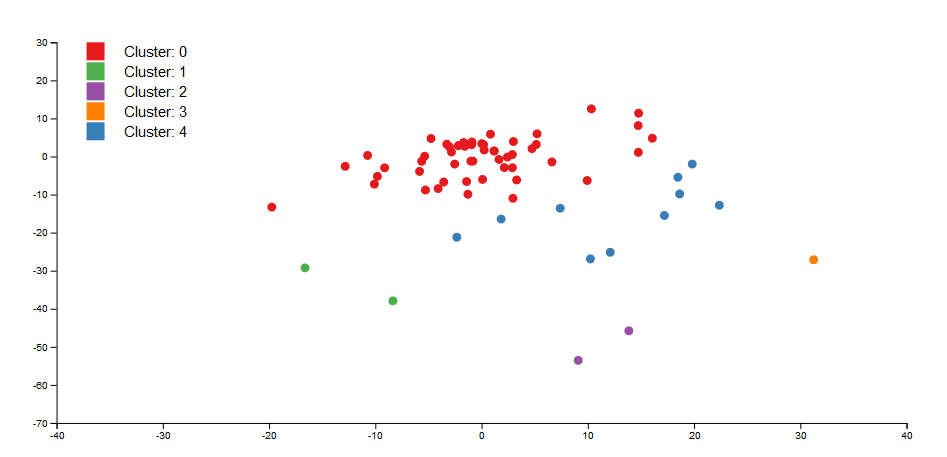
\includegraphics[width=80mm,scale=1]{mds.png}
	\caption{MDS Scatter Plot}
\end{figure}
\noindent From the picture above, it is interesting to notice that teams of the same cluster are very close to each other.
In fact, considering Germany and Brazil they are very close to each other because when a team  won the World Cup the other was on top 5 and viceversa. More in detail, in 1958, 1970 and 2002 when Brazil won the World Cup, Germany was respectively in fourth, third and second position. 
While when two teams are far from each other means they got different performances during the same competition, in fact, Italy is far from Germany because for example when Italy won the World Cup in 1938, Germany went out in eights of final while when Germany won in 1974, Italy did not even pass the group stage.
\subsection{K-means}
We applied Truncated-SVD and K-means to the original dataset (not the one produced by Mds).\\We have decided to truncate up to 15 components because the explained variance with this number of components is above 90\%.\\We have applied 5-means because the average inertia (intra-cluster scatter) per cluster with this value of k is rather low.\\To plot the cluster we have colored the points in the Mds space, and we gave to the cluster the following interpretation:
\begin{enumerate}
\item belonging to a given cluster is driven not only by the number of medals won by a team, but also how similar the teams performed over the years : this is why Italy has won a lot but it is not in the same cluster of Brazil and Germany.
\begin{figure}[H]
	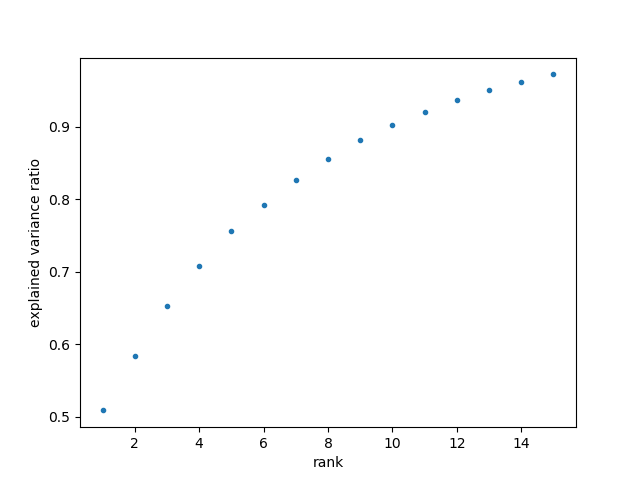
\includegraphics[width=60mm,scale=0.7]{explained-variance.png}
	\caption{explained variance for SVD}
\end{figure} 
\begin{figure}[H]
	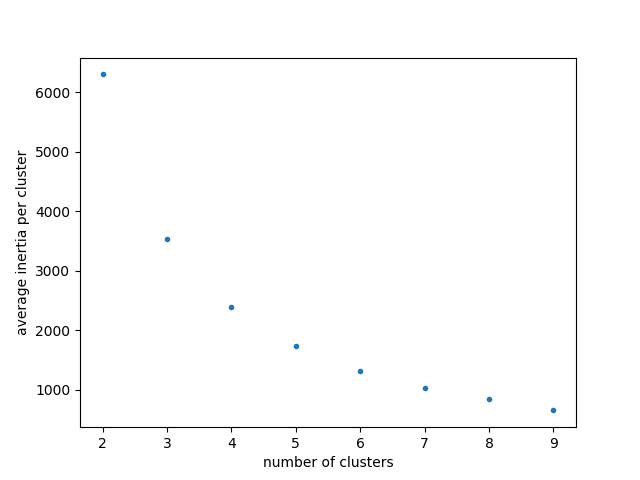
\includegraphics[width=60mm,scale=0.7]{average-inertia.png}
	\caption{average inertia in k-means}
\end{figure} 
\end{enumerate}

\subsection{Additional work}
As suggested by Professor Marco Angelini, we added a new interaction in the reverse way. \\
In particular, from the Scatter Plot, is possible to mouse over  one team that will be plotted in the Radar Chart and Line Chart.\\
In this way it is possible to quickly compare the selected teams in the Choropleth Map with that team.
\begin{thebibliography}{9}

\bibitem{Scott Murray}
  Scott Murray,
  \textit{Interactive Data Visualization for the Web},
  O'Reilly Media,
  2nd edition,
  2017.
  
\bibitem{mbostock}
  \textit{ https://bl.ocks.org/mbostock} 

\bibitem{mbostock}
  \textit{https://www.kaggle.com/martj42/international-football-results-from-1872-to-2017} 

\bibitem{mbostock}
  \textit{https://stats.stackexchange.com/questions/43099/how-to-explain-the-connection-between-svd-and-clustering}
 \bibitem{mbostock}
\textit{https://www.fifa.com/fifa-world-ranking/ranking-table/men/}
\bibitem{mbostock} 
  \textit{https://d3js.org/}
\bibitem{mbostock}
\textit{https://scrapy.org/}



\end{thebibliography}
\end{document}
